\documentclass[t]{beamer}

\usepackage[english]{babel}
\usepackage[utf8]{inputenc}
\usepackage{graphicx}
\usepackage{changepage}
\usepackage{hyperref}

\hypersetup{
   unicode=true,
   hidelinks
}
\usetheme{imbe}
%%%%%%%%%%%%%%%%%%%%%%%%%%%%%%%%%%%%%%%%%%%%%%%%%%%%%%%%%%%%%%%%%
% DOCUMENT/TITLE PAGE INFO
%%%%%%%%%%%%%%%%%%%%%%%%%%%%%%%%%%%%%%%%%%%%%%%%%%%%%%%%%%%%%%%%%
\title[opti4Abq - A tentative tutorial/documentation]{opti4Abq, a python toolbox to run abaqus in an optimisation loop}
\subtitle{A tentative tutorial/documentation}
\date{\today}
\author{Marl\`ene Mengoni}

\institute[IMBE]{
	\href{mailto:m.mengoni@leeds.ac.uk}{m.mengoni@leeds.ac.uk}\\
}
%%%%%%%%%%%%%%%%%%%%%%%%%%%%%%%%%%%%%%%%%%%%%%%%%%%%%%%%%%%%%%%%%
% MAIN CONTENT
%%%%%%%%%%%%%%%%%%%%%%%%%%%%%%%%%%%%%%%%%%%%%%%%%%%%%%%%%%%%%%%%%
\begin{document}

\titleframe

% Concept
\section[Background]{Concept}
\begin{frame}{Concept: FE model calibration}
One use of FE models is to calibrate some unknown variable(s) - e.g. material parameters - to match known experimental data.

To do so, one need: 
\begin{itemize}
\item 1 or more FE models that are parametrised with the unknown variable(s) to calibrate;
\item a way to run FE models with parameters automatically;
\item a way to process FE models so that it outputs the value(s) of interest;
\item the corresponding experimental data;
\item a process to vary the parameters for the FE to match the experimental data.
\end{itemize}

\end{frame}


\begin{frame}{Concept: FE model calibration}
One use of FE models is to calibrate some unknown variable(s) - e.g. material parameters - to match known experimental data.

To do so, one need: 
\begin{itemize}
\item {\color{blue} 1 or more FE models that are parametrised with the unknown variable(s) to calibrate};
\item {\color{darkgreen} a way to run FE models with parameters automatically};
\item {\color{orange} a way to process FE models so that it outputs the value(s) of interest};
\item the corresponding experimental data;
\item {\color{darkgreen} a process to vary the parameters for the FE to match the experimental data}.
\end{itemize}

{\color{blue} Abaqus scripting interface}; {\color{darkgreen} \href{https://github.com/mengomarlene/opti4Abq}{opti4Abq} toolbox framework};

{\color{orange} e.g. \href{https://github.com/mengomarlene/postPro4Abq}{postPro4Abq} toolbox}
\end{frame}

\section[]{}
\begin{frame}{opti4Abq}%table of content
  \myToc
\end{frame}
% data preparation
\section{Data Preparation}
\begin{frame}[fragile]{Data Preparation}
\begin{itemize}
\item 1 or more FE models = 1 or more Python files defining an Abaqus job and post-processing function
\item the corresponding experimental data = 1 or more text files containing the experimental data formatted as the post-processing of the FE models formats its output
\end{itemize}

NOTES:
\begin{itemize}
\item[] all Python files must be stored in 1 folder [\texttt{pyPath}]
\item[] all experimental files must be stored in 1 folder [\texttt{expPath}]
\item[] (can be same folder!)
\item[]
\item[] \texttt{pyPath} must contain an empty file called \texttt{\_\_init\_\_.py}
\end{itemize}
\end{frame}
\begin{frame}[fragile]{Data Preparation - python file}

The file name of the python file is the model {\color{red} identifier}.
The file must contain:
\begin{enumerate}
\item an abaqus job creation (function of parameters):
\begin{verbatim}
if __name__ == '__main__':
    import sys
    nbParam = 2
    paramToOpti = list()
    for arg in range(nbParam):
       paramToOpti.insert(0,float(sys.argv[-1-arg]))
    job = jobCreation(paramToOpti) 
    job.submit()
    job.waitForCompletion()
\end{verbatim}
\item A function  (called \texttt{postPro}) that reads the odb and writes a file called
    \texttt{output.dat} with output of interest
\end{enumerate}
\end{frame}
\begin{frame}[fragile]{Data Preparation - data file}

The experimental data relative to each model must be stored in a text file called \texttt{{\color{red} identifier}.dat}

\vfill

The type of data supported is:
\begin{enumerate}
\item a function  y = y(x)
\hspace{.5cm} 0.0 0.0 \hspace{.2cm} e.g. displacement/load data

in 2 column x y
\hspace{1.15cm} 0.1 0.1

\hspace{3.8cm} 0.2 0.5

\hspace{3.8cm} 0.9 2.3

\item a list of 1D values
\hspace{.75cm} 0.0  \hspace{.2cm} e.g. $\sigma_{VM}$ at known locations

\hspace{3.8cm} 0.1

\hspace{3.8cm} 0.2

\hspace{3.8cm} 0.9
\item a scalar
\hspace{2.3cm} 10.0  \hspace{.2cm} e.g. structure stiffness
\end{enumerate}
\end{frame}
% opti preparation and run
\section[Optimisation process]{Optimisation preparation and run}
\begin{frame}[fragile]{opti4Abq object}
\begin{itemize}
\item preparing the optimisation

\verb|import opti4AbqTools.Opti4AbqClass as optiTools|

\verb|myOpti = optiTools.Opti4Abq(p0, expPath, pyPath)|\\[5pt]

\verb|p0| is a Python list with the initial guess of the parameter values

\item Running the optimisation\\[5pt]

if type of data is scalar:
\begin{verbatim}
       p,fVal,info = myOpti.runScalar()
\end{verbatim}
else:
\begin{verbatim}
       p,fVal,info = myOpti.run()
\end{verbatim}
\end{itemize}
\end{frame}


\begin{frame}[fragile]{opti4Abq methods}
\begin{itemize}
\item\verb|myOpti.setBounds(low = boundsL,high = boundsH)|

where \verb|boundsL| and \verb|boundsH| are the lowest and highest authorised values of the parameters

\item\verb|myOpti.setResidualsAsAbsolute(True)|

will try to minimise the absolute difference between the experimental and computational data (default is set at False: relative difference is used)

\item\verb|myOpti.setVerbose(True)|

writes plenty of things and save values at each iterations (for some opti algorithms)

\end{itemize}
\end{frame}

\begin{frame}{Gradient-based optimisation}
\centering\vfill
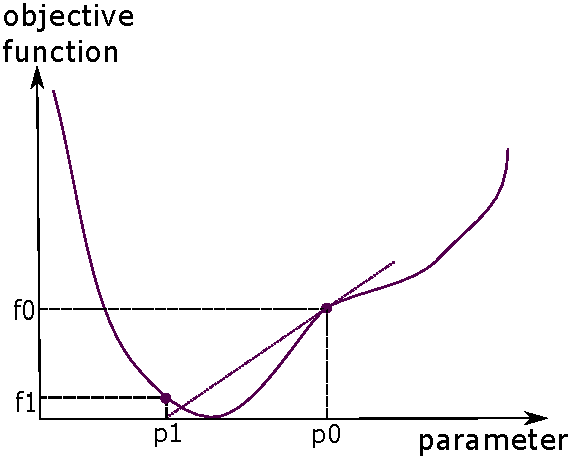
\includegraphics[height=.85\textheight,keepaspectratio]{figures/gradientBased.pdf}
\vfill
\end{frame}
\begin{frame}[fragile]{opti4Abq options}

\verb|myOpti.setOptions(options)|:
\vskip20pt
\begin{adjustwidth}{-1.5em}{-1.5em}
\begin{tabular}{ll}
\textbullet\ control end of process&\\
\verb|options['maxIter']= 10|&max number of iterations\\
\verb|options['tol']= 1e-4|&tolerance on the parameter\\
&variation\\
\verb|options['ftol']= options['tol']*1e-4|&tolerance on the function\\
\verb|options['gtol']= options['tol']*1e-4|&tolerance on the gradient\\
\\
\textbullet\ control step to evaluate gradient&\\
\verb|options['eps']= 1e-4|&step for the jacobian
\end{tabular}
\end{adjustwidth}

\end{frame}
% what it does
\section{What it does}
\begin{frame}{Objective function}
\hfill

\begin{block}{scalar data}
difference or error between data and FE
\end{block}

\begin{block}{1D data}
RMS difference or error between data and FE
\end{block}

{\setlength{\tabcolsep}{.1em}
\begin{block}{(x,y) data}
\begin{tabular}{rl}
\multicolumn{2}{l}{RMS difference or error between data and FE}\\[0.5ex] 
  BUT& unlikely to have same sampling rate in x\\
  $\longrightarrow$ first& resample to same (smallest) sampling rate in x\\
\end{tabular}
\end{block}}
If Nb models $>1$, RMS error/difference over all models of previous value.
\end{frame}

\begin{frame}{Optimisation methods (interfaced from \href{https://docs.scipy.org/doc/}{scipy})}
\hfill

\begin{block}{scalar data \& 1 parameter}
\begin{tabular}{ll}
\href{https://docs.scipy.org/doc/scipy/reference/generated/scipy.optimize.minimize_scalar.html}{Brent method} & whether  parameter bounded or not
\end{tabular}\end{block}

\begin{block}{other data \& 1 parameter}
\begin{tabular}{ll}
\href{https://docs.scipy.org/doc/scipy/reference/generated/scipy.optimize.minimize.html
}{L-BFGS-B method} &bounded parameter\\[.5ex]
\href{https://docs.scipy.org/doc/scipy/reference/generated/scipy.optimize.minimize.html}{Conjugate gradient method} &non-bounded
\\
\end{tabular}\end{block}
\begin{block}{any data \& $>1$ parameters}
\begin{tabular}{ll}
\href{https://docs.scipy.org/doc/scipy/reference/generated/scipy.optimize.least_squares.html}{Trust Region Reflective method} &bounded parameters\\[.5ex]
\href{https://docs.scipy.org/doc/scipy/reference/generated/scipy.optimize.leastsq.html}{Levenberg-Marquadt method} (MINPACK) &non-bounded
\end{tabular}\end{block}
\end{frame}

% output
\section{Outputs}
\begin{frame}{Outputs}
\texttt{p,fVal,info = myOptiProcess.run()}

\begin{itemize}
\item \texttt{p}: output parameters
\item \texttt{fVal}: value of the objective function
\item \texttt{info}: a dictionary of information:
\begin{itemize}
\item \texttt{info['funcalls']}: number of function evaluation that were required
\item \texttt{info['task']}: an output message by the optimisation process
\item \texttt{info['grad']}: the value of the jacobian
\end{itemize}
\item[]
\item[+] all Abaqus files (and output of interest) of the last run (in \texttt{workspace})
\item[+] for some of the algorithms, intermediate \texttt{p} and \texttt{fVal} values into text files (in \texttt{results}) [if \texttt{verbose==True}]
\end{itemize}
\end{frame}

\begin{frame}{Limitations}

\begin{itemize}
\item all parameters need to have values of the same order
\item all python files need to be stored in same folder (hence need second copy in other directory if running on subset of models) and only python files that are models can be in that folder (in particular no tools module)
\item all python files defining abaqus jobs need to be launchable with
  \texttt{abaqus cae nogui=myPythonFile.py}
  
  ? may be an issue with user subroutines
\item all models need to have the same type of data
\item not easily portable on HPC environments with SGE queues!
\item currently only limited gradient-based opti algorithms interfaced
\item \dots [probably plenty of others!]
\end{itemize}

\end{frame}

% example
\section{Example}
\begin{frame}{Examples}
\vfill

\begin{enumerate}
\item \texttt{scalar1Param} directory:  scalar function, 1 parameter, bounded
\item[]
\item \texttt{1D2Param} directory: 1D function, 2 parameters, bounded
\item[]
\item \texttt{xy2Param} directory: (x,y) function, 2 parameters, bounded
\end{enumerate}
\vfill
\begin{block}{Note}
All example files are set with absolute paths to search for external modules/files that need setting up and all use the postPro4Abq toolbox to post-process the data!
\end{block}
\end{frame}
% admin
\section[Citation]{Requirements and Acknowledging the toolbox}
\begin{frame}{Requirements}

\vfill
The toolbox is built for Python 2.x and Abaqus $\>6.13$ (not been tested on anterior versions).

Requires scipy 0.18 or above, with numpy 1.11 or above.
\vfill
I personally use the anaconda distribution of Python (conda v.4.3.11, Python v.2.7.13)
\vfill
The toolbox has been tested on Windows platform only with no guarantee to work on any other OS
\vfill

\end{frame}
\begin{frame}{Acknowledging the toolbox}
\vfill
The toolbox is available in \href{https://github.com/mengomarlene/opti4Abq}{github} with latest stable/documented release on zenodo\\[.5cm]
    
To reference opti4Abq in publications, please cite both of the following:
{\footnotesize
\begin{enumerate}
\item Mengoni M., Luxmoore B.J., Jones A.C., Wijayathunga V.N., Broom N.D. \& Wilcox R.K. (2015)
\href{http://dx.doi.org/10.1016/j.jmbbm.2015.03.028}{"Derivation of inter-lamellar behaviour of the intervertebral disc annulus."} Journal of the Mechanical Behavior of Biomedical Materials, v 48, 164–172

\item Mengoni M. (2017) "opti4Abq (v.2.0), a generic python code to run Abaqus in an optimisation loop". \url{http://dx.doi.org/10.5281/zenodo.580475}

\item[\color{black} e.g.]  {\it The opti4Abq toolbox$^{[1,2]}$ using the L-BFGS-B algorithm implemented in SciPy (Python 2.7, www.python.org) was used in this work.}
\end{enumerate}
}

\end{frame}

\setbeamertemplate{headline}{\vskip50pt}
\setbeamertemplate{footline}{}
\begin{frame}[noframenumbering]{Thanks!}

\vfill\hfill
\parbox[t]{.95\textwidth}{

This work was funded through WELMEC, a Centre of Excellence in Medical Engineering funded by the Wellcome Trust and EPSRC, under Grant number 088908/Z/09/Z and through EPSRC Grant EP/K020757/1 and ERC Grant StG-2012-306615
\begin{center}
\begin{tabular}[t]{c}
\\

\includegraphics[height=.2\paperheight,keepaspectratio]{figures/EPSRC.pdf}

\includegraphics[height=.2\paperheight,keepaspectratio]{figures/LOGO-ERC.pdf}\\
\\

\includegraphics[height=.07\paperheight,keepaspectratio]{figures/WellcomeTrust.pdf}
\end{tabular}
\end{center}

}
\end{frame}

\end{document}
